%\section{微弱扰动在可压缩流体中的传播}
\subsection{微弱扰动源静止不动($v=0$)}
\begin{frame}{微弱扰动源静止不动($v=0$)}
  \begin{figure}
 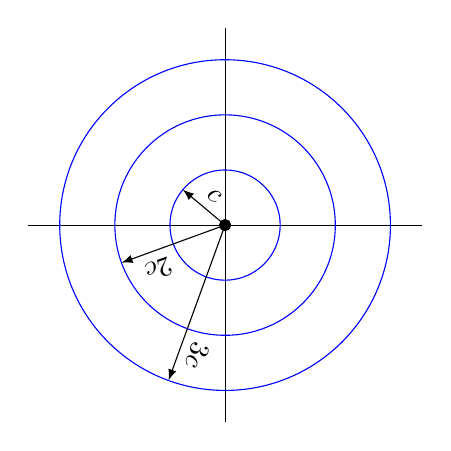
\begin{tikzpicture}
   \draw (-2.5,0) -- (2.5,0);
   \draw (0,-2.5) -- (0,2.5);
   \draw[fill] (0,0) circle (2pt);
   \uncover<2->{
     \draw[blue] (0,0) circle (0.7cm);
   \draw[-latex] (0,0) -- node[midway,above,rotate=-40]{$c$} ++(140:0.7cm);
 }
 \uncover<3->{
   \draw[blue] (0,0) circle (1.4cm);
   \draw[-latex] (0,0) -- node[pos=0.7,above,rotate=200]{$2c$} ++(200:1.4cm);
 }
 \uncover<4->{
   \draw[blue] (0,0) circle (2.1cm);
   \draw[-latex] (0,0) -- node[pos=0.8,above,rotate=250]{$3c$} ++(250:2.1cm);
 }
 \end{tikzpicture}
 \end{figure}
\end{frame}

\subsection{微弱扰动源作亚声速匀速运动($v<c$)}
\begin{frame}{微弱扰动源作亚声速匀速运动($v<c$)}
  \begin{figure}
 \begin{tikzpicture}
   \draw (-2.5,0) -- (2.5,0);
   \draw (0,-2.5) -- (0,2.5);
   \uncover<2->{
   \draw[fill] (0,0) node[anchor=north]{$0$} circle (2pt);
   \draw[fill] (-0.3,0) node[anchor=north]{$1$} circle (2pt);
 }
 \only<2>{
   \draw[blue] (0,0) circle (0.7cm);
   \draw[-latex] (0,0) -- node[pos=0.5,above,rotate=60]{$c$} ++(60:0.7cm);
 }
 \uncover<3->{
   %\draw[fill] (-0.3,0) node[anchor=north]{$1$} circle (2pt);
   \draw[fill] (-0.6,0) node[anchor=north]{$2$} circle (2pt);
 }
 \only<3>{
   \draw[blue] (0,0) circle (1.4cm);
   \draw[blue] (-0.3,0) circle (0.7cm);
   \draw[-latex] (0,0) -- node[pos=0.8,above,rotate=60]{$2c$} ++(60:1.4cm);
   \draw[-latex] (-0.3,0) -- node[pos=0.7,above,rotate=60]{$c$} ++(60:0.7cm);
 }
 \uncover<4->{
   \draw[fill] (-0.9,0) node[anchor=north]{$3$} circle (2pt);
   \draw[blue] (0,0) circle (2.1cm);
   \draw[blue] (-0.3,0) circle (1.4cm);
   \draw[blue] (-0.6,0) circle (0.7cm);
   \draw[-latex] (0,0) -- node[pos=0.8,above,rotate=60]{$3c$} ++(60:2.1cm);
   \draw[-latex] (-0.3,0) -- node[pos=0.7,above,rotate=60]{$2c$} ++(60:1.4cm);
   \draw[-latex] (-0.6,0) -- node[pos=0.5,above,rotate=60]{$c$} ++(60:.7cm);
 }
 \uncover<5->{
 \begin{scope}[xshift=5.5cm]
   \draw[fill] (0.3,0) circle (2pt);
   \draw[blue] (0.9,0) circle (2.1cm);
   \draw[blue] (0.6,0) circle (1.4cm);
   \draw[blue] (0.3,0) circle (0.7cm);
   \draw[-latex] (0.9,0)++(0:2.1) -- node[midway,anchor=south west]{$c+v$} ++(0.6,0);
   \draw[-latex] (0.9,0)++(180:2.1) -- node[midway,anchor=south east]{$c-v$} ++(180:0.4);
 \end{scope}
 }
 \end{tikzpicture}
 \end{figure}
\end{frame}

\subsection{微弱扰动源作声速匀速运动($v=c$)}
\begin{frame}{微弱扰动源作声速匀速运动($v=c$)}
  \begin{figure}
 \begin{tikzpicture}
   \draw (-2.5,0) -- (2.5,0);
   \draw (0,-2.5) -- (0,2.5);
   \uncover<2->{
   \draw[fill] (0,0) node[anchor=north]{$0$} circle (2pt);
   \draw[fill] (-0.7,0) node[anchor=north]{$1$} circle (2pt);
 }
 \only<2>{
   \draw[blue] (0,0) circle (0.7cm);
   \draw[-latex] (0,0) -- node[pos=0.5,above,rotate=60]{$c$} ++(60:0.7cm);
 }
 \uncover<3->{
   %\draw[fill] (-0.7,0) node[anchor=north]{$1$} circle (2pt);
   \draw[fill] (-1.4,0) node[anchor=north]{$2$} circle (2pt);
 }
 \only<3>{
   \draw[blue] (0,0) circle (1.4cm);
   \draw[blue] (-0.7,0) circle (0.7cm);
   \draw[-latex] (0,0) -- node[pos=0.8,above,rotate=60]{$2c$} ++(60:1.4cm);
   \draw[-latex] (-0.7,0) -- node[pos=0.7,above,rotate=60]{$c$} ++(60:0.7cm);
 }
 \uncover<4->{
   \draw[fill] (-2.1,0) node[anchor=north]{$3$} circle (2pt);
   \draw[blue] (0,0) circle (2.1cm);
   \draw[blue] (-0.7,0) circle (1.4cm);
   \draw[blue] (-1.4,0) circle (0.7cm);
   \draw[-latex] (0,0) -- node[pos=0.8,above,rotate=60]{$3c$} ++(60:2.1cm);
   \draw[-latex] (-0.7,0) -- node[pos=0.7,above,rotate=60]{$2c$} ++(60:1.4cm);
   \draw[-latex] (-1.4,0) -- node[pos=0.5,above,rotate=60]{$c$} ++(60:.7cm);
 }
 \uncover<5->{
 \begin{scope}[xshift=5cm]
   \draw[fill] (-0.7,0) circle (2pt);
   \draw[blue] (1.4,0) circle (2.1cm);
   \draw[blue] (0.7,0) circle (1.4cm);
   \draw[blue] (0.0,0) circle (0.7cm);
   \draw[-latex] (1.4,0)++(0:2.1) -- node[midway,anchor=south west]{$2c$} ++(0.7,0);
 \end{scope}
 }
 \end{tikzpicture}
 \end{figure}
\end{frame}

\subsection{微弱扰动源作超声速匀速运动($v>c$)}
\begin{frame}{微弱扰动源作超声速匀速运动($v>c$)}
  \begin{figure}
 \begin{tikzpicture}
   \draw (-3.7,0) -- (2.2,0);
   %\draw (0,-4.5) -- (0,2.5);
   \uncover<2->{
   \draw[fill] (0,0) node[anchor=north]{$0$} circle (2pt);
   \draw[fill] (-1.2,0) node[anchor=north]{$1$} circle (2pt);
 }
 \only<2>{
   \draw[blue] (0,0) circle (0.7cm);
   \draw[-latex] (0,0) -- node[pos=0.5,above,rotate=60]{$c$} ++(60:0.7cm);
   \draw (-1.2,0) coordinate (O) -- ++(36:2.5);
   \draw (-1.2,0) -- ++(-36:2.5);
 }
 \uncover<3->{
   \draw[fill] (-2.4,0) node[anchor=north]{$2$} circle (2pt);
 }
 \only<3>{
   \draw[blue] (0,0) circle (1.4cm);
   \draw[blue] (-1.2,0) circle (0.7cm);
   \draw[-latex] (0,0) -- node[pos=0.8,above,rotate=60]{$2c$} ++(60:1.4cm);
   \draw[-latex] (-1.2,0) -- node[pos=0.7,above,rotate=60]{$c$} ++(60:0.7cm);
   \draw (-2.4,0) coordinate (O) -- ++(36:3.5);
   \draw (-2.4,0) -- ++(-36:3.5);
 }
 \uncover<4->{
   \draw[fill] (-3.6,0) node [anchor=north]{$3$} circle (2pt);
   \draw[blue] (0,0) circle (2.1cm);
   \draw[blue] (-1.2,0) circle (1.4cm);
   \draw[blue] (-2.4,0) circle (0.7cm);
   \draw[-latex] (0,0) -- node[pos=0.8,above,rotate=60]{$3c$} ++(60:2.1cm);
   \draw[-latex] (-1.2,0) -- node[pos=0.7,above,rotate=60]{$2c$} ++(60:1.4cm);
   \draw[-latex] (-2.4,0) -- node[pos=0.5,above,rotate=60]{$c$} ++(60:.7cm);
   \draw[red] (-3.6,0) coordinate (O) -- node[pos=0.4,rotate=36,anchor=south west]{马赫锥(线)} ++(36:3.5) coordinate (A);
   \draw[red] (-3.6,0) -- ++(-36:3.5) coordinate (B);
   \draw[dashed, red, thin] (-2.4,0) -- ++(126:0.7);
   \tkzMarkAngle[arc=l, size=0.4](B,O,A)
   \tkzLabelAngle[pos=0.6](B,O,A){$2\alpha$}
   \node at (-3.6, -3.0) [anchor=south west]{$\displaystyle \sin{\alpha}=\frac{c}{v}=\frac{1}{\mathrm{Ma}}$};
   \node at (-3.6, 1.8) [anchor=south west]{寂静区域};
 }
 \uncover<5->{
   \begin{scope}[xshift=6cm]
   \draw[fill] (-3.6,0) circle (2pt);
   \draw[blue] (0,0) circle (2.1cm);
   \draw[blue] (-1.2,0) circle (1.4cm);
   \draw[blue] (-2.4,0) circle (0.7cm);
   \draw[red] (-3.6,0) coordinate (O) -- ++(36:3.5);
   \draw[red] (-3.6,0) -- ++(-36:3.5);
   \draw[-latex] (0,0)++(0:1.5) -- node[midway,anchor=south]{$c+v$} ++(0.7,0);
   \end{scope}
 }
 \end{tikzpicture}
 \end{figure}
\end{frame}
